\newpage
\section{\text{k-Fold }Cross Validation}
This approach involves randomly dividing the set of observations into $k$ groups, or folds, of approximately equal size. The first fold is treated as a validation set, and the method is fit on the remaining $k-1$ folds.
\\
Library function used: \texttt{\href{https://scikit-learn.org/stable/modules/generated/sklearn.model_selection.cross_val_score.html}{cross\_val\_score}} from \texttt{sklearn.model\_selection}
\\
Note that the model hyperparameters used here are in their default settings
\begin{figure}[h!]
    \centering
    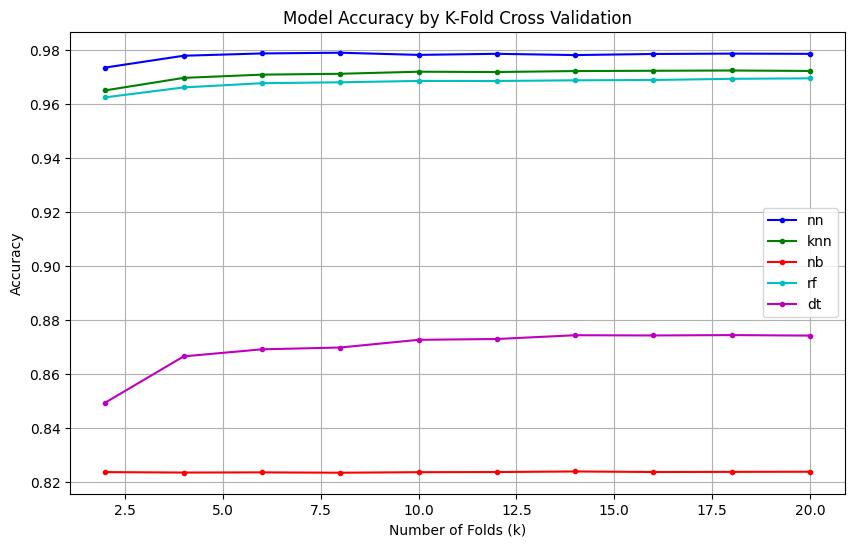
\includegraphics[width=1\linewidth]{images/kfold_CV.png}
    \caption{\text{k-Fold} Cross Validation on all models}
\end{figure}